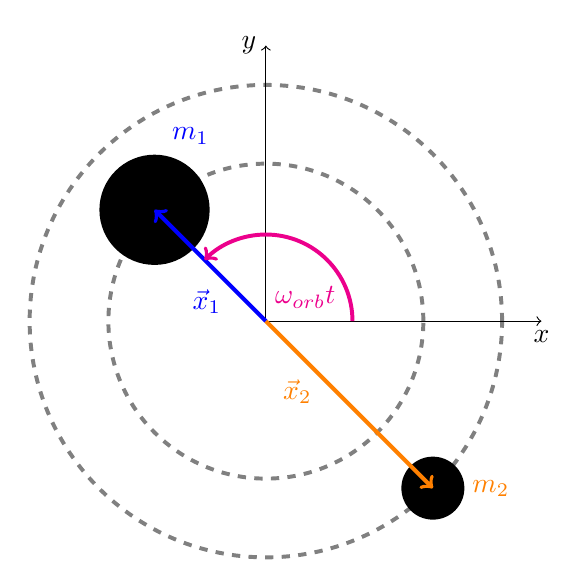
\begin{tikzpicture}
    \draw[dashed, gray, line width=0.5mm] (0, 0) circle(2);
    \draw[dashed, gray, line width=0.5mm] (0, 0) circle(3);
    \fill (2.121, -2.121) circle (0.4);
    \fill (-1.414, 1.414) circle (0.7);
    \draw[->] (0, 0) -- (0, 3.5); 
    \draw[->] (0, 0) -- (3.5, 0); 
    \draw[->, blue, line width=0.5mm] (0, 0) -- (-1.414, 1.414); 
    \draw[->, orange, line width=0.5mm] (0, 0) -- (2.121, -2.121); 
    \node[left, blue] at (-0.6, 2.35) {$m_1$};
    \node[right, orange] at (2.5, -2.121) {$m_2$};
    \node[left] at (0, 3.5) {$y$};
    \node[below] at (3.5, 0) {$x$};
    \node[orange] at (0.4, -0.9) {$\vec{x}_2$};
    \node[blue] at (-0.75, 0.25) {$\vec{x}_1$};
    \node[magenta] at (0.5, 0.3) {$\omega_{orb}t$};
    \draw [->, magenta, line width=0.5mm] (1.1, 0) arc[start angle=0, end angle=135, radius=1.1];
\end{tikzpicture}